\begin{figure}[t]
 \centering
    \subfloat[CNN Layers\label{fig:layers}]{%
      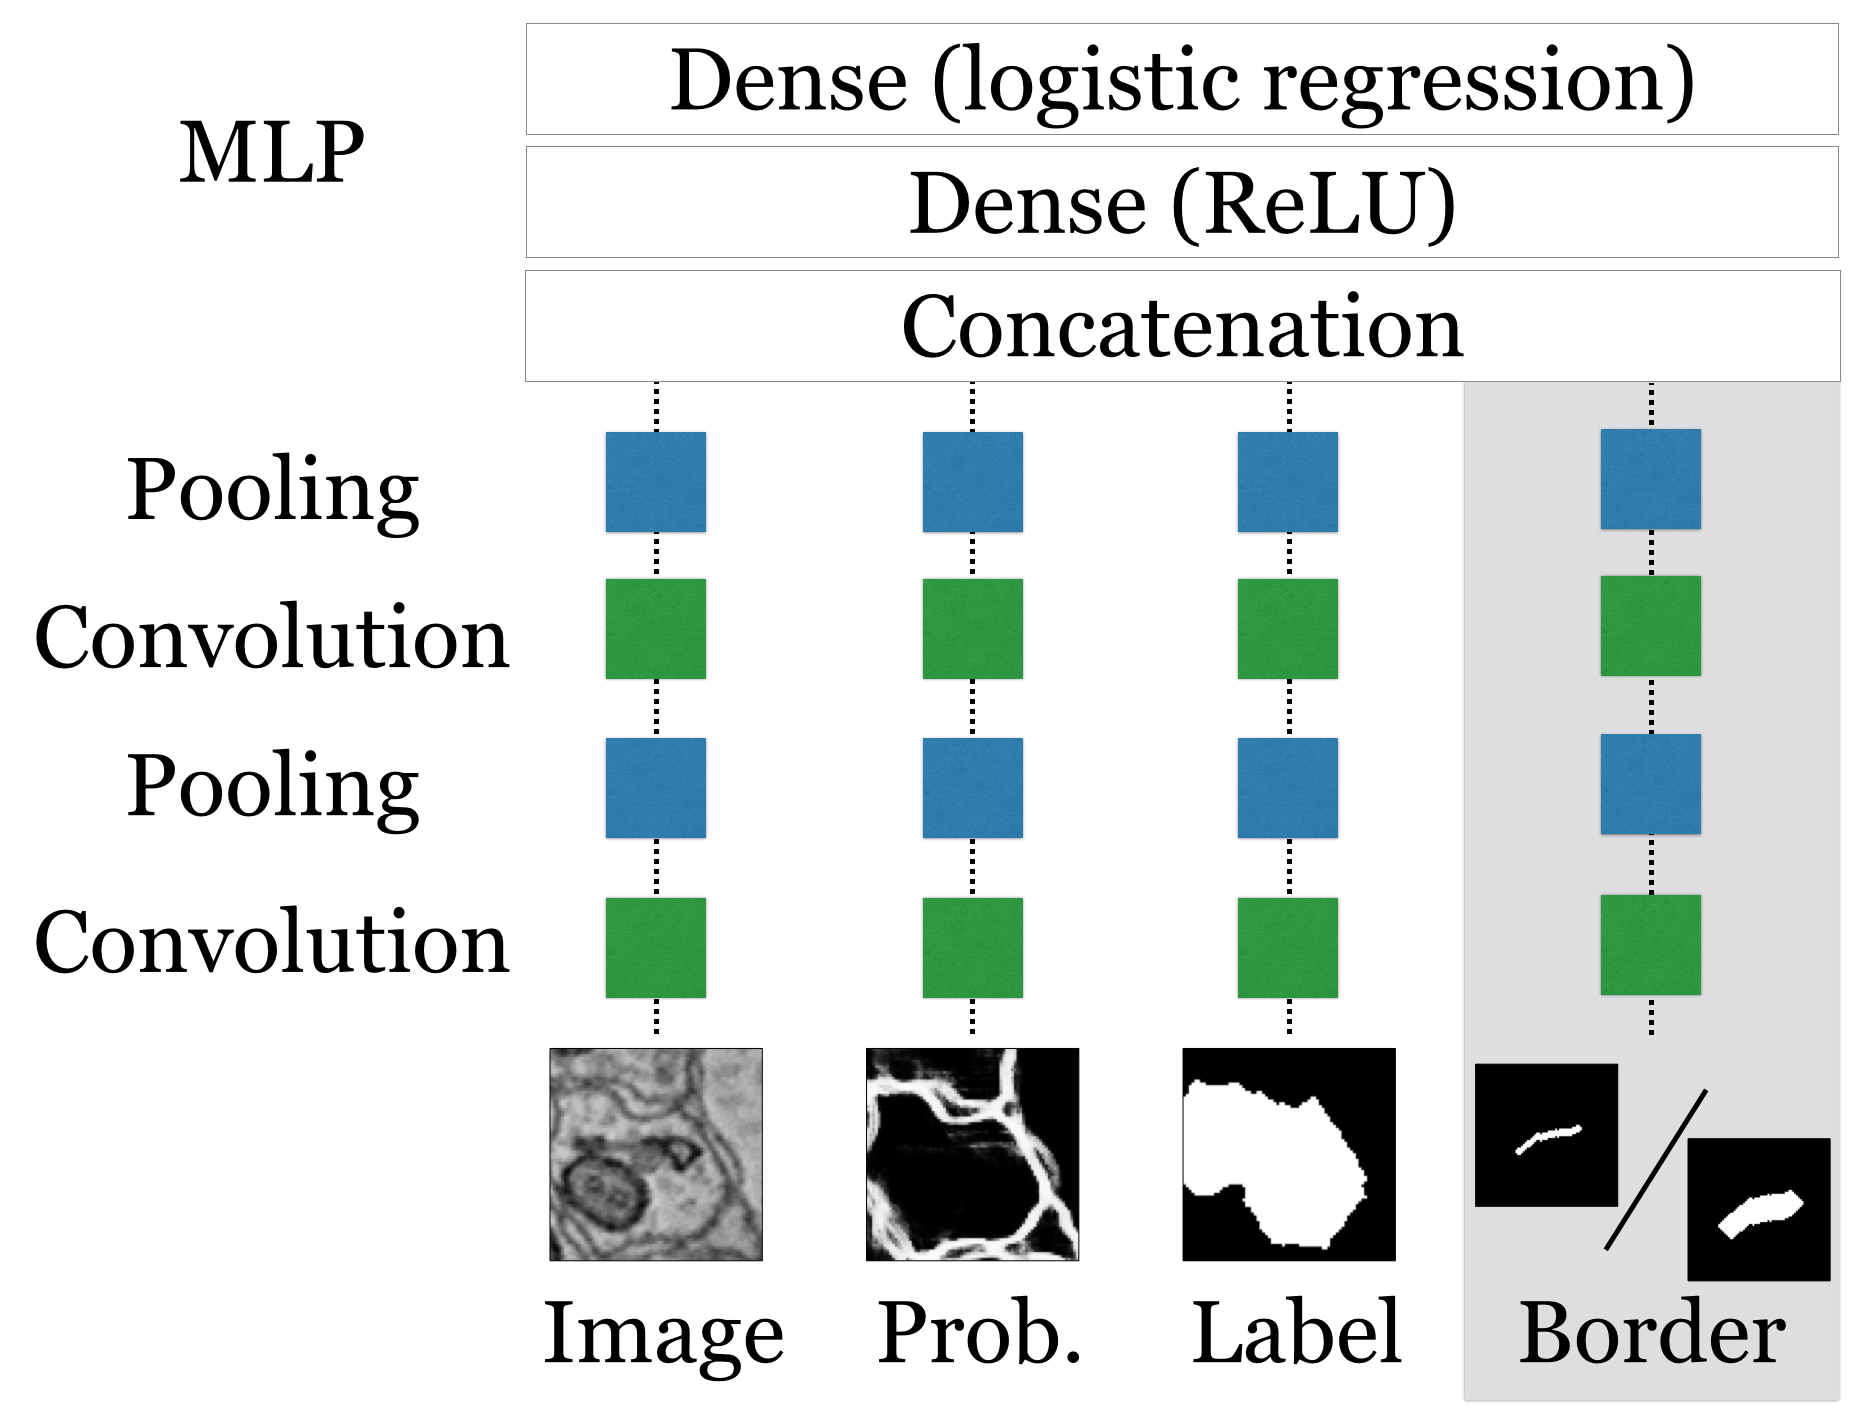
\includegraphics[width=0.9\textwidth]{gfx/network.png}
    }

    \subfloat[Network configurations\label{fig:networks}]{%
      \includegraphics[width=0.9\textwidth]{gfx/network_inputs.png}
    }
	\caption{(a) Our network architecture with up to four input channels, each with two convolutional and two pooling layers. MergeNet includes four separate input channels and RGBANet uses a 4-channel input. (b) We trained three different network configurations with three and four inputs: A) image, boundary map probability, and merged binary mask; B) A configuration extended with a small border mask, to focus on the specific boundary in question; C) A configuration extended with a large border mask.}

\end{figure}

\section{Method}
%Paragraph one: Overview of the method. What are the high level steps taken to build the system? What are the key techniques used within the system?
We build a split error classifier using a convolutional neural network (CNN) to check the boundaries of an existing automatic segmentation. For each boundary, the CNN provides a probability that points sampled along the boundary caused a split error. For each boundary, we sample up to 10 decision points, where the decision points are spread evenly over the boundary length, so long as their context windows do not overlap. These probabilities are then weighted by the length of the boundary within the context over the total boundary length, and averaged. A greedy algorithm then merges neighboring regions sequentially, starting with the highest probability score. Following each merge, neighboring boundaries are re-evaluated for split errors. Correcting a split error is as simple as merging the two bordering labels.

Identification and correction of merge errors is more challenging, because we must look inside segmentation regions for missing or incomplete boundaries and then propose the correct boundary. However, we can reuse the same trained CNN for this task. For each segmentation label, we generate 30 potential boundaries through the region by placing watershed seed points at opposite sides of the label boundary and generating the corresponding split. Then, we check to see whether any potential edge is classified as a split error. If the CNN detects a boundary with a very low split error score, then the boundary should have been in the segmentation and the region is a candidate for a merge error.
%\JT{Candidate for figure - this potential boundary generation is a bit tricky to follow.}\VKF{Maybe put some more candidates into Figure 1 as examples?}



%\begin{figure}[t]
%\centering
%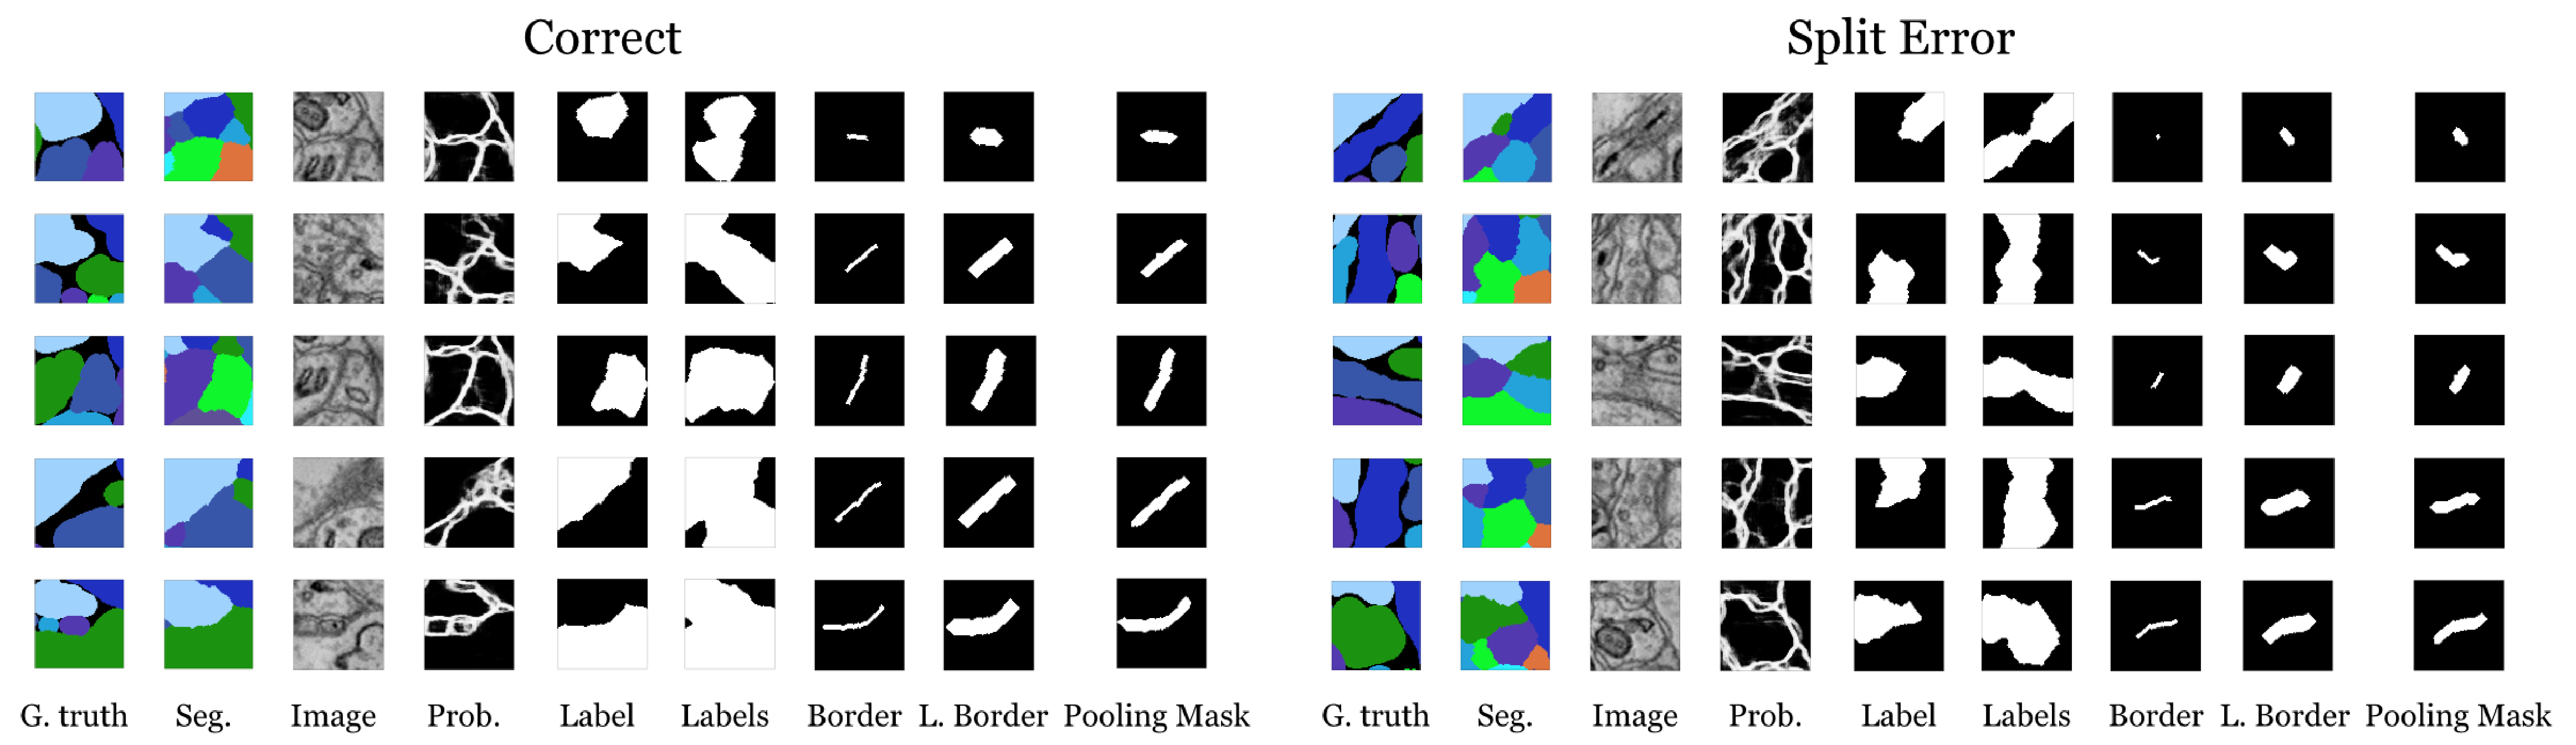
\includegraphics[scale=.15]{gfx/patches.pdf}
%\caption{\JT{NEW CAPTION PLEASE.}}
%\label{fig:patches}
%\end{figure}




\subsection{Convolutional Neural Network Design}
%Paragraph: What is the rationale behind our network design? Why do we think this will work over other approaches?
To train a CNN for split error detection we take multiple channels of context information of the boundary into consideration for the decision making process. We pass multiple inputs into the CNN windowed around a particular decision point or pixel: the input grayscale image patch, the corresponding boundary probability map patch, and two corresponding binary mask patches for the segmented regions at either side of the boundary. Following Bogovic et al.~\cite{BogovicHJ13}, these two masks can be combined into a single mask with comparable performance (configuration A, Fig.~\ref{fig:networks}). The network then leverages these multiple input patches to identify and correct errors made by the previous membrane detection network and automatic segmentation pipeline.

One way to combine these inputs is to treat them as a 4-channel input, so that alignment between the input image and the segmentation masks are not lost throughout the convolutions. We refer to this approach as \textit{RGBANet}. However, training a boundary-classifying network can be difficult due to rigid ground-truth segmentations, which often differ substantially from automatic segmentation regions in ambiguous extra-cellular space. To cope with this variation, our network is based on multiple separate input channels (Fig.~\ref{fig:layers}). Each of the input patches is connected individually to a 2-layer network, with each layer consisting of convolutional and pooling layers. The output of these networks is then combined by a fully connected multi-layer perceptron (MLP) with one hidden layer and a two class logistic regression output layer. The intuition for this multiple input channel approach is that we want to allow variation in the input and masks independently, to accommodate potential error, and then for the hidden layers to discover appropriate combinations of the relevant features learned separately for the different input channels. We refer to this approach as \textit{MergeNet}.

To better direct both networks to train on the true boundary edge, which in many cases is missing from the boundary probability map and hence is the cause of merge errors, we additionally pass as input a second binary mask. This mask contains the true boundary edge (configuration B, Fig.~\ref{fig:networks}). To consider slight edge ambiguities, we also test a version of this network where the true boundary mask has been dilated by 5 pixels (configuration C).

% \VKF{DELETE RIGHT? Another change is in the pooling layer itself. Bogovic et al.~\cite{BogovicHJ13} designed an unsupervised learning approach for agglomerative clustering of oversegmentations, using dynamic pooling of features extracted around objects and boundaries to increase performance. Inspired by their call for a supervised learning equivalent, we integrate a pooling layer into our CNN which is similar in spirit to their unsupervised approach. Instead of conventional max- or avg-pooling where a sliding window is equally applied to the whole output of the convolutional layer, our dynamic pooling only averages outputs within a region of interest. We implemented both pooling methods and compared them ???} 


%  
%    \begin{subfig}[b]{0.5\textwidth}
%        \includegraphics[scale=.15]
%        \caption{CNN Layers}
%        \label{fig:layers}
%    \end{subfigure}
%    \begin{subfigure}[b]{0.5\textwidth}
%        \includegraphics[scale=.15]
%        \caption{Different Network Configurations}
%        \label{fig:networks}
%    \end{subfigure}    
%\missingfigure{Network architecture figure}


\subsection{Training}
To train the network, we use the blue 3-cylinder mouse cortex volume of Kasthuri et al. \cite{kasthuri2015saturated} (2048 x 2048 x 300 voxels). The tissue is dense mammalian neuropil from layers 4 and 5 of the S1 primary somatosensory cortex of a healthy mouse. The resolution of our data set is $3\, nm$ per pixel, and the section thickness is $30\, nm$. 
%\VKF{For the initial automatic segmentation, we train an existing pipeline on a similar data set}. 
A manually-labeled expert segmentation is available as a ground truth for the entire data set. We use the first 250 sections of the data for training and validation (split 0.25) and the last 50 for testing. To generate training data, we identify correct regions and split errors in the automatic segmentation by intersecting with the ground truth regions. From these regions, we sample 266,088 correct regions and 266,088 split error patches. As patch size, we defined $75 x 75$ pixels to cover $\approx80\%$ of all boundaries in our segmentation output. 
%#   Training data:
%#   Patch size: (75,75)
%#   79828 correct splits
%#   79828 split errors
%#   rotated 90,180,270 degrees after each epoch
%
%#   validation data: 7464 correct splits + 7464 split errors
%#   test data: 5748 correct splits + 5748 split errors


\begin{figure*}
%\ffigbox[][\textwidth]{
%\begin{floatrow}

\includegraphics[width=.5\textwidth]{gfx/roc_plot.pdf}


\begin{tabular}{l rrrr}
\toprule
Network & Validation loss & Test acc. ~(\%) & Prec./Recall & \hspace{0.1cm} F1 Score \\
\midrule
A. MergeNet: Image + boundary prob. + seg. label & 0.073 & 0.906 & 0.906/0.906 & 0.907 \\
B. MergeNet: A config. + small border overlap ($d=1$) & 0.076 & 0.905 & 0.907/0.905 & 0.908 \\
C. MergeNet: A config. + large border overlap ($d=5$) & 0.07 & 0.908 & 0.908/0.908 & 0.909 \\
D. RGBANet: A. config. & 0.058 & 0.895 & 0.895/0.895 & 0.894 \\
E. RGBANet: B. config. & 0.054 & 0.907 & 0.907/0.907 & 0.908 \\
F. RGBANet: C. config. & 0.058 & 0.905 & 0.905/0.905 & 0.904\\
%A. Image + boundary prob. + seg. label & 0.3853 & 0.4163 & 81.15 \\
%B. A config. + small border overlap($d=1$) & 0.3798 & 0.3843 & 82.34\\
%C. A config. + large border overlap ($d=5$) &  0.3703 & 0.3919 & 83.02\\
%Bogovic et al. + small border overlap($d=1$) & 0.379833 & 0.384347 & 82.34\\
%Bogovic et al. + large border overlap ($d=5$) &  0.370280 & 0.391911 & 83.02\\
\bottomrule
\end{tabular}

%\end{floatrow}
%}{
 \caption{Network design training evaluation. Adding an extra channel containing a binary mask of just the border slightly increases performance in both network configurations. We take configuration MergeNet C to evaluate VI against human performance.}
 \label{fig:trainingperformance}
%}
\end{figure*}

We train our networks using the following parameters: learning rate $lr=0.03$ (iteratively decreasing until $lr=0.00001$), momentum $m=0.9$ (iteratively increasing until $m=0.999$), filter size $fs=13\times13$ and number of filters $fn=16$ for MergeNet, and number of filters $fn_1=64, fn_2=48$ for RGBANet. This results in ~1.5 million parameters for all network configurations. For regularization we use dropout layers after each pooling layer with $p=0.2$. We assume that the training has converged if the validation loss does not decrease for 50 epochs. The network is specified using the deep learning libraries Lasagne and Theano \cite{Bastien-Theano-2012}, and trained on a Tesla K40m graphics card.

Figure \ref{fig:trainingperformance} presents validation loss function scores (cross validation), test accuracy percent as well as precision/recall and F1 scores. Based on these performances, we select configuration MergeNet C to evaluate against human performance in a VI improvement experiment.







%\subsection{Error Discovery and Correction}

%\VKF{Our experiments have shown that the best average probability threshold to stop this process is in the range ($p_t=.7-1.0$) not sure what to do with this, I think this is from the test data? Do we need this still? At the moment it sounds weird}.
%\subsection{Merge Error Discovery and Correction}

%With the intuition that merge errors are caused by the failure to correctly detect a boundary, we can use the inverse probability of the split error classifier to help discover merge errors. For each segmentation region, we generate 30 possible splits across the region using watersheds seeded from the region boundary (Fig.~\ref{fig:merge_error}). Then, each candidate split is tested using our split error classifier. If the candidate split is 

%\VKF{Do we need this? If it stays we should not just hope. I think it can go if we publish the code. Further, we dilate the region segmentation by a fixed amount ($d=20$) prior to running watershed, hoping that one of the generated split edges clings to the boundary of the cell and then follows the correct splitting edge. To remove pixels that then overlap the boundary of the cell, we perform erosion by a fixed amount ($e=5$).} 

%
%\begin{table}
%\begin{tabular}{ll}
%\toprule
%Parameter & Value \\
%\midrule
%one & \\
%two & \\
%three & \\
%\bottomrule
%\end{tabular}
%\caption{This is a table of parameters. This is not very interesting, but it's easier to read than in the body text and putting everything together helps the reader quickly assess.}
%\end{table}